\chapter{Исследование метода имитации отжига}
\label{chapter:simulated_annealing}

В данном разделе представлены улучшения метода имитации отжига (simulated
annealing) и экспериментальные результаты, полученные данным методом для шифров
DES, MacGuffin и ГОСТ~28147-89. Исследнованы новые критерии вычислительного
поиска криптографически стойких S-блоков. На основе усовершенствованных весовых
коэффициентов ценовых функций поиска предлагается дальнейшее развитие метода
имитации отжига. В основу предлагаемых функций стоимости положены спектральные и
корреляционные свойства недвоичных криптографических функций, математический
аппарат которых предложен в \cite{Kuznetsov}. Проведены оценки быстродействия
формирования нелинейных узлов замен методом имитации отжига для шифров MacGuffin
и ГОСТ~28147-89 в сравнении с методом случайной генерации.

\section{Ценовые функции и их улучшение}

Метод имитации отжига, изложенный в разделе~\ref{section:simulated_annealing},
основывается на постепенном улучшении текущего нелинейного узла замен оценивая
эффект внесённых изменений на каждом шаге формирования при помощи cost (ценовой)
функции.

Рассмотрим процедуры формирования функций стоимости ценовых функций,
используемые для синтеза S-блоков через спектральные характеристики булевых
функций, введем соответствующие функции стоимости для синтеза S-блоков через
спектры недвоичных криптографических функций.

Пусть функция $F(x):GF^{n}(2)\rightarrow GF^{m}(2)$ задает S-блок размерности $n \times m$.
Пусть для $\beta \in GF^{m}(2)$, $F_{\beta}(x) = \beta_{1}f_{1}(x) \xor \ldots \xor \beta_{m}f_{m}(x)$, "---
линейная комбинация m выходов S-блока $F$. Тогда $\hat{F}_{\beta}(\omega), r_{\beta}(s)$
"--- значения преобразования Уолша-Адамара и значения автокорреляции для каждой булевой функции $f_{\beta}$.

Поскольку нелинейность булевой функции
\begin{equation}NL_f=\frac{1}{2}(2^n - \max_{\omega}|\hat{F}(\omega)|),\end{equation}
то задача повышения нелинейности может быть представлена как задача минимизации
абсолютного максимального значения коэффициента Уолша-Адамара. Изначально в
задачах синтеза S-блоков по критерию высокой нелинейности для метода имитации
отжига использовалась следующая функция стоимости \cite{Clark1}:
\begin{equation}cost(f) = WHT_{max}(f) = \max_{\omega}|\hat{F}(w)|.\end{equation}

Поскольку задача понижения автокорреляции представляется как задача минимизации
максимального значения автокорреляционной функции, то cost функция в дальнейших
исследованиях приняла следующий вид \cite{Clark1}:
\begin{equation}cost(f) = AC(f) = \max_{s \neq 0}|\sum_{x}\hat{f}(x)\hat{f}(x
\xor s)|=\max_{s \neq 0}|\hat{r}(s)|.\end{equation}

Обычно в многокритериальных задачах применяется следующий подход: вычисляется
сумма отдельных cost функций (по различным критериям), умноженных на весовые
коэффициенты. Тогда cost функция в задаче синтеза S-блока с высокой
нелинейностью и низкой автокорреляцией принимает вид \cite{Clark1}:
\begin{equation}cost(f) = \alpha \cdot WHT_{max}(f) + \beta \cdot
AC(f).\end{equation}

Далее были разработаны улучшенные функции, которые основывались на следующем
положении. 

Известно, что равенство Парсеваля
\begin{equation}\sum(\hat{F}(\omega))^2 = 2^{2n}\end{equation}
ограничивает $WHT_{max}(f) = \max_{\omega}|\hat{F}(\omega)|$ значением равным
как минимум $2^{n/2}$. Данная граница достигается тогда, когда выполняется
равенство $\hat{F}(\omega) = 2^{n/2}$ для каждого $\omega$. Когда значение
некоторого коэффициента $|\hat{F}(\omega)|$ меньше этой идеальной границы,
теорема Парсеваля утверждает, что другие значения коэффициентов
$|\hat{F}(\omega)|$ должны быть выше этой границы. Таким образом, попытка
ограничить отдаленность абсолютных значений коэффициентов Уолша-Адамара от
данной границы является возможным средством достижения высокой нелинейности.
Спектры некоторых функций содержат все значения (по модулю), равные этой
идеальной границы. Такие функции называются бент-функциями. 

Помимо обладания наивысшей возможной нелинейностью эти функции имеют нулевую
автокорреляцию. Следовательно, функция стоимости
\begin{equation}\label{eq:cost1}cost(f) = \sum_{\omega \in GF^{n}(2)}||\hat{F}(\omega)| - 2^{n/2}|^R\end{equation}
является возможным подходом к оптимизации нелинейности и автокорреляции. В виду
несбалансированности бент-функций приведенная функция стоимости cost может быть
улучшена для нахождения сбалансированных криптографических функций. В \cite{Clark1} было
введено обобщение функции стоимости (\ref{eq:cost1}), которое приняло следующий вид 
\begin{equation}\label{eq:cost2}cost(f) = \sum_{\omega \in GF^{n}(2)}||\hat{F}(\omega)| - X|^R.\end{equation}

Параметры X и R, называемые весовыми коэффициентами, обеспечивают свободу для
экспериментирования и поиска оптимальных значений. 

По аналогии с функциями стоимости относительно спектра Уолша-Адамара вида (\ref{eq:cost2}),
функции стоимости относительно спектра автокорреляционной функции имеют
следующий вид:
\begin{equation}\label{eq:cost3}cost(f) = \sum_{s \in GF^{n}(2)}||r(s)| - X|^R.\end{equation}

Традиционно, ценовые функции применяются для оптимизации отдельной булевой
функции. Для всего же нелинейного узла замен cost функции, основанные на спектре
Уолша-Адамара, можно обобщить следующим образом \cite{Clark1}:
\begin{equation}\label{eq:cost4}cost(f) = \sum_{\beta \in GF^{m}(2)}\sum_{\omega \in GF^{n}(2)}||\hat{F}_{\beta}(\omega)| - X|^R\end{equation}
и аналогично для cost функций, основанных на автокорреляционном спектре:
\begin{equation}\label{eq:cost5}cost(f) = \sum_{\beta \in GF^{m}(2)}\sum_{s \in GF^{n}(2)}||r_{\beta}(s)| - X|^R.\end{equation}

Для оптимизации по критериям нелинейности и автокорреляции в \cite{Kavut} использовалась
следующая функция стоимости:
\begin{equation}\label{eq:cost6}\begin{split}cost(f) &= \sum_{\beta \in GF^{m}(2)}\sum_{\omega \in GF^{n}(2)}||\hat{F}_{\beta}(\omega)| - X_1|^{R_1} \\
&+ \sum_{\beta \in GF^{m}(2)}\sum_{s \in GF^{n}(2)}||r_{\beta}(s)| - X_2|^{R_2}.\end{split}\end{equation}

Изначально в исследованиях использовались функции стоимости вида (\ref{eq:cost3}),
(\ref{eq:cost4}), с заменой спектральных коэффициентов Уолша-Адамара и
коэффициентов автокорреляционных спектров булевых функций на предложенные в \cite{Kuznetsov}
коэффициенты соответствующих спектров недвоичных функций.

Дальнейшие исследования состояли в совершенствовании функций стоимости (критерия
поиска криптографических функций), которое основывается на следующем положении.
Известно, что при оптимизации криптографической функции по нелинейности и
автокорреляции она по своим спектральным характеристикам (спектру корреляции с
линейными функциями и автокорреляционному спектру) стремится к спектральным
характеристикам бент-функций, что и было использовано в предыдущих работах
\cite{Clark1,Kavut} при разработке функций вида (\ref{eq:cost1}) -
(\ref{eq:cost6}). В тоже время, очевидным недостатком такого подхода является
использование одного (фиксированного) значения статического коэффициента, к
которому стремятся все спектральные значения оптимизируемой криптографической
функции. При этом значения спектральных коэффициентов идеальной функции (или
бент-функции) состоят из двух возможных значений для булевых функций, и из трех
значений для введенных в \cite{Kuznetsov} недвоичных функций. При введении же
дополнительных ограничения на сбалансированность, количество возможных значений
спектральных коэффициентов еще более возрастает. 

При разработке новых функций стоимости предлагается в (\ref{eq:cost2}) -
(\ref{eq:cost6}) заменить статический весовой коэффициент X на так называемые
динамические весовые коэффициенты, т.е. весовые коэффициенты, принимающие
различные значения для различных входных индексов спектра. В данной работе в
качестве значений динамических весовых коэффициентов используются спектральные
значения бент-функций. Предлагаемые функции стоимости имеют вид:
\begin{gather}
\label{eq:cost7}cost(f) = \sum_{\omega \in GF^{n}(2)}|\hat{F}_{\beta}(\omega)| - \hat{B}(\omega)|^R, \\
\label{eq:cost8}cost(f) = \sum_{s \in GF^{n}(2)}|r_{F}(s)| - r_{B}(s)|^R, \\
\label{eq:cost9}\begin{split}cost(f) &= \sum_{\omega \in GF^{n}(2)}|\hat{F}_{\beta}(\omega)| - \hat{B}(\omega)|^{R_1} \\
&+ \sum_{s \in GF^{n}(2)}|r_{F}(s)| - r_{B}(s)|^{R_2},\end{split}
\end{gather}
где $\hat{B}(\omega), r_{B}(s)$ "--- спектральные значения нелинейности и автокорреляции случайной недвоичной
бент-функции $B$.

Таким образом, в основе предлагаемого вычислительного метода синтеза регулярных
нелинейных узлов замен симметричных криптоалгоритмов лежит применение
математического аппарата недвоичных криптографических функций \cite{Kuznetsov}, методов
корреляционного и спектрального анализа, а также предложенных в данной работе
усовершенствованных ценовых функций (\ref{eq:cost7}) - (\ref{eq:cost9}), с
использованием динамических весовых коэффициентов $\hat{B}(\omega), r_{B}(s)$.
Усовершенствованный таким образом метод имитации отжига позволяет, как показано
ниже, реализовать вычислительный поиск регулярных узлов замен c требуемыми
показателями нелинейности и автокорреляции.


\section{Экспериментальных исследования формирования нелинейных узлов замен}
\label{section:sboxes_design}

Для подтверждения достоверности и обоснованности полученных теоретических
результатов в данной работе проведены экспериментальные исследования
эффективности предлагаемого вычислительного метода синтеза регулярных нелинейных
узлов замен. Первая часть исследований была проведена с использованием спектров
недвоичных функций со статическими весовыми коэффициентами в функциях стоимости
(\ref{eq:cost4}) - (\ref{eq:cost6}) метода имитации отжига, вторая часть
исследований "--- с использованием динамических коэффициентов в функциях
стоимости (\ref{eq:cost7}) - (\ref{eq:cost9}).

Путём экспериментальных исследований были выбраны следующие параметры для всех
последующих вычиследний:

\begin{itemize}

    \item $\alpha = 0.95$ "--- параметр геометрического охлаждения;

    \item $MIL = 500$ "--- число шагов, предпринимаемых во внутреннем цикле;

    \item $MaxIL = 300$ "--- максимальное число внутренних циклов поиска;

    \item $MUL = 50$ "--- максимальное число последовательных непродук- тивных
    внутренних циклов;

    \item количество пробегов алгоритма для каждого набора параметров равно 10.

\end{itemize}

В ходе экспериментов с функциями стоимости вида (\ref{eq:cost4}) -
(\ref{eq:cost6}) использовались различные значения статических коэффициентов $X$
и фиксированное значение $R = 3$.

Формировались S-блоки размерностей $8 \times 2$, $4 \times 4$, $6 \times 4$. Узлы замен выходной
размерности 4 представлялись через одну недвоичную функцию над GF(24). 

Полученные экспериментальные результаты для S-блоков $8 \times 2$ приведены в
табл.~\ref{table:sbox_8x2}. Лучший полученный результат выделен жирным шрифтом.

Как видно из полученных результатов использование функций стоимости с
динамическими весовыми коэффициентами позволило повысить показатели стойкости
нелинейности и автокорреляции формируемых узлов замен. 

В табл.~\ref{table:compare_sbox_8x2} приведено сравнение полученных результатов с лучшими
известными результатами, использующих традиционный подход описания S-блока в
виде совокупности компонентных булевых функций
\cite{Millian1,Millian2,Clark1,Laskari,Tesar}.  Как видно из приведенной
таблицы, полученные экспериментальные результаты предлагаемым методом с
использованием функций стоимости на основе спектров недвоичных функций и
статических весовых коэффициентов хорошо согласуются с экспериментальными
результатами вычислительных методов традиционного подхода.  Использование
динамических весовых коэффициентов позволило получить лучшие известные на
сегодняшний день результаты для S-блоков $8 \times 2$.

\begin{table}[ht]
    \caption{Криптографические свойства S-блоков $8 \times 2$}
    \label{table:sbox_8x2}
    \begin{tabular}{| m{5.75cm} | m{1cm} | m{1cm} | m{1cm} | m{1cm} |}
        \hline
        \multirow{2}{*}{\vbox{Способ построения спектров}} &
        \multicolumn{2}{m{5cm}}{Статические коэффициенты} &
        \multicolumn{2}{|m{5cm}|}{Динамические коэффициенты} \\ \cline{2-5}
                        & NL    & AC    & NL    & AC \\ \hline
        WHT, ср.        & 110   & 56    & 114   & 24 \\ \hline
        WHT, худш.      & 108   & 56    & 116   & 24 \\ \hline
        ACT, ср.        & 110   & 48    & 114   & 24 \\ \hline
        ACT, худш.      & 112   & 40    & 114   & 24 \\ \hline
        WHT+ACT, худш.  & 112   & 40    & 114   & 24 \\ \hline
        WHT+ACT, ср.    & 112   & 40    & 114   & 24 \\ \hline
    \end{tabular}
\end{table}

\begin{table}[ht]
    \caption{Сравнение с результатами традиционного подхода, синтез S-блоков $8 \times 2$}
    \label{table:compare_sbox_8x2}
    \begin{tabular}{| m{10.75cm} | C{2.5cm} | C{2.5cm} |}
        \hline
        \centering{Метод синтеза}           & NL    & AC \\ \hline
        Случайная генерация                 & 108   & 56 \\ \hline
        Генетические алгоритмы              & 110   & 48 \\ \hline
        Имитация отжига (булевы функции)    & 114   & 32 \\ \hline
        Имитация отжига (недвоичные функции)& 112   & 40 \\ \hline
        Имитация отжига (недвоичные функции, динамические весовые коэффициенты) & 116 & 24 \\ \hline
    \end{tabular}
\end{table}

В табл.~\ref{table:sbox_4x4_6x4} приведены лучшие полученные результаты для S-блоков $4 \times 4$ и $6 \times 4$. 

Как видно из приведенной таблицы, применение предлагаемого подхода позволяет
повысить нелинейность формируемых S-блоков $6 \times 4$. Подобные S-блоки (размерности
$6 \times 4$) применяются в DES-подобных шифрах. 

\begin{table}
    \caption{Криптографические свойства S-блоков $4 \times 4$, $6 \times 4$}
    \label{table:sbox_4x4_6x4}
    \begin{tabular}{| C{2cm} | m{11.25cm} | C{1cm} | C{1cm} |}
        \hline
        S-блок          & Метод имитации отжига     & NL    & AC \\ \hline
        $4 \times 4$    & Булевы функции            & 4     & 8  \\ \hline
        $4 \times 4$    & Функции над GF(24)        & 4     & 8  \\ \hline
        $6 \times 4$    & Булевы функции            & 22    & 24 \\ \hline
        $6 \times 4$    & Функции над GF(24)        & 24    & 24 \\ \hline
    \end{tabular}
\end{table}

Как показал проведенный анализ S-блоки DES по своим криптографическим
показателям нелинейности NL и автокорреляции AC далеки от оптимальных (см.
данные для S1-S8 в табл.~\ref{table:sbox_6x4}). Разработанный вычислительный
метод предлагается использовать для синтеза DES-подобных S-блоков с улучшенными
криптографическими показателями стойкости (в табл.~\ref{table:sbox_6x4} приведены характеристики
формируемых узлов замен S1*-S8*).

\begin{table}[ht]
    \caption{Исследование криптографических свойств регулярных узлов замен $6 \times 4$}
    \label{table:sbox_6x4}
    \begin{tabular}{| m{9.25cm} | C{2cm} | C{2cm} | C{2cm} |}
        \hline
        S-блок      & NL        & AC        & $DDT_{max}$ \\ \hline
        S1          & 14        & 48        & 16        \\ \hline
        S2          & 16        & 56        & 16        \\ \hline
        S3          & 16        & 48        & 16        \\ \hline
        S4          & 16        & 64        & 16        \\ \hline
        S5          & 12        & \bf 40    & \bf 16    \\ \hline
        S6          & \bf 18    & 48        & 16        \\ \hline
        S7          & 14        & 52        & 16        \\ \hline
        S8          & 16        & 48        & 16        \\ \hline
        \bf S1*-S8* & \bf 24    & \bf 24    & \bf 10    \\ \hline
    \end{tabular}
\end{table}

Следует отметить, что для обеспечения стойкости DES-подобных шифров к
дифференциальному и линейному криптоанализу сформированные S-блоки необходимо
оценивать не только по показателям нелинейности и автокорреляции, но и c учетом
других критериев, учитывающих саму структуру шифра \cite{Kwangjo}. В этом смысле
оценка эффективности формируемых S-блоков с учетом ограничений, накладываемых
особенностями основных преобразований БСШ, а также апробация полученных
результатов являются перспективным направлением дальнейших исследований.

\section{Критерии построения нелинейных узлов замен DES}
\label{section:des_criteria}

В \cite{Coppersmith} описаны следующие критерии, которым должны соответствовать
нелинейные узлы замен в шифре DES:

\begin{itemize}

    \item (S-1) Каждый нелинейный узел замен имеет шесть входных и четыре
    выходных бит;

    \item (S-2) Ни один выходной бит узла замен не должен быть слишком близок к
    линейной функции входных бит, это значит, выбирая любое положение выходного
    бита и любое подмножество из шести бит на входе позиций, доля данных, для
    которых этот выходной бит равен XOR этих входных биты не должно быть близко
    к 0 или 1, а скорее должны быть около 1/2;

    \item (S-3) Если зафиксировать самый левый и правый входные биты, выходные
    биты должны быть различны для всех вохможных 4-хбитовых выходов;

    \item (S-4) Если два входа в нелинейный узел замен отличаются ровно на один
    бит, то выходные значения должны отличаться не менее, чем на два бита;

    \item (S-5) Если два входа в нелинейный узел замен отличаются ровно в двух
    средних битах, то выходы должны отличаться не менее, чем в двух битах;

    \item (S-6) Если два входа в нелинейный узел замен отличаются в их первых
    двух битах и идентичны в их последних двух битах, то два выхода не должны
    совпадать.

\end{itemize}

Данные критерии были реализованы в утилите, описанной в
разделе~\ref{chapter:program}, и
использовались для дальнейшей оценки формируемых нелинейных узлов замен в
разделе~\ref{section:des_research}.

\section{Экспериментальные исследования DES-подобных шифров}
\label{section:des_research}

В данном разделе будут рассмотрены экспериментальные результаты влияния
нелинейных узлов замен на сложность дифференциального и линейного криптоанализа
DES и MacGuffin шифров. Для сравнения будут использованы рекомендуемые к шифрам
и сформированные методом имитации отжига нелинейные узлы замен.

Исследования нелинейных узлов замен размерностью $6 \times 4$, которые
используются в DES, были представленны в разделе~\ref{section:sboxes_design},
однако в данном разделе к требованиям, выдвигаемым к формируемым нелинейным
узлам замен, добавятся критерии, выдвигаемые непосредственно к узлам замен,
применяемых в шифре DES. Данные критерии~\cite{Coppersmith} были рассмотрены в
разделе~\ref{section:des_criteria}, также реализованы в утилите, описанной в
разделе~\ref{chapter:program}.

Однако, сформировать нелинейные узлы замен, отвечающие одновременно нашим
критериям и критериям, выдвигаемыми авторами шифра DES, в отведённые сроки не
удалось. Это может также свидетельствовать о необходимости замены полностью
случайной генерации начального состояния и случайных перестановок на
детерменированные методы, разработанные специально для нелинейных узлов замен
DES.

Таким образом, для дальшейших исследований был взят шифр MacGuffin. Данный шифр
интересен тем, что имеет такую же размерность S-блоков, $6 \times 4$, однако
имеет не $2^4$ различных выходов, а только $2^2$. Также шифр MacGuffin
изначально разрабатывался в исследовательских целях, что делает его
привлекательным для изучения.

Шифр MacGuffin не выдвигает никаких требований к нелинейным узлам замен,
кроме размерности $6 \times 4$ и выходным значениям из $GF(2^2)$.

В ходе исследований были получены и проанализированы такие показатели:
\begin{itemize}
    \item нелинейность (NL);
    \item автокорреляция (AC);
    \item $\Delta$-разность (максимум в таблице дифференциалов);
    \item лучшая линейная аппроксимация (максимальное абсолютное значение в таблице линейных аппроксимаций).
\end{itemize}

Для увеличения стойкости необходимо максимизировать нелинейность и
минимизировать автокорреляцию, дифференциальную и линейнную характеристики.

Как можно убедиться из таблиц~\ref{table:sbox_MacGuffin} и
\ref{table:sbox_MacGuffin_annealed}, метод имитации отжига дал оптимальные
нелинейные узлы замен, которые по всем показателям дал значительное улучшение
оцениваемых показателей.

\begin{table}
    \caption{Криптографические свойства исходных S-блоков шифра MacGuffin}
    \label{table:sbox_MacGuffin}
    \centering\begin{tabular}{| m{2cm} | m{2cm} | m{2cm} | m{4.4cm} | m{4.4cm} |}
        \hline
        S-блок  & NL    & AC    & $\Delta$-разность & Лучшая линейная аппроксимация \\ \hline
        1       & 18    & 32    & 34                & 14                        \\ \hline
        2       & 18    & 40    & 36                & 14                        \\ \hline
        3       & 18    & 48    & 34                & 14                        \\ \hline
        4       & 16    & 64    & 32                & 16                        \\ \hline
        5       & 20    & 32    & 32                & 12                        \\ \hline
        6       & 20    & 48    & 32                & 12                        \\ \hline
        7       & 18    & 48    & 34                & 14                        \\ \hline
        8       & 20    & 40    & 32                & 12                        \\ \hline
    \end{tabular}
\end{table}

\begin{table}
    \caption{Криптографические свойства S-блоков для шифра MacGuffin, сформированных методом имитации отжига}
    \label{table:sbox_MacGuffin_annealed}
    \centering\begin{tabular}{| m{9cm} | m{0.8cm} | m{0.8cm} | m{1.9cm} | m{2.1cm} |}
        \hline
        S-блок                                          & NL    & AC    & $\Delta$-разность & Лучшая линейная аппроксимация \\ \hline
        2, 2, 2, 1, 3, 3, 3, 3, 0, 3, 0, 2, 0, 0, 1, 0 
        0, 3, 2, 0, 3, 2, 0, 1, 1, 2, 3, 3, 2, 0, 3, 2 
        2, 2, 1, 3, 1, 1, 0, 2, 2, 0, 2, 3, 1, 3, 1, 0 
        1, 1, 3, 1, 1, 3, 2, 1, 0, 3, 2, 1, 0, 0, 0, 1  & 24    & 16    & 24            & 8                 \\ \hline
        2, 1, 1, 2, 1, 2, 2, 2, 0, 0, 3, 0, 3, 1, 2, 0 
        3, 0, 3, 3, 3, 1, 1, 3, 0, 0, 2, 0, 0, 0, 2, 3 
        2, 3, 1, 3, 3, 1, 3, 2, 2, 2, 0, 3, 3, 1, 1, 1 
        2, 2, 3, 1, 0, 0, 0, 1, 0, 1, 0, 3, 2, 1, 2, 1  & 24    & 16    & 24            & 8                 \\ \hline
        2, 0, 2, 0, 1, 3, 0, 3, 1, 0, 2, 0, 1, 1, 2, 2 
        2, 0, 3, 2, 3, 3, 3, 3, 2, 3, 0, 1, 1, 2, 3, 0 
        3, 0, 0, 2, 1, 0, 3, 1, 2, 2, 2, 1, 1, 1, 2, 0 
        1, 1, 0, 3, 3, 1, 0, 2, 3, 1, 0, 3, 2, 3, 1, 0  & 24    & 16    & 24            & 8                 \\ \hline
        1, 1, 1, 0, 2, 0, 3, 2, 1, 0, 2, 2, 1, 2, 0, 1 
        3, 3, 3, 1, 2, 3, 3, 1, 3, 2, 3, 2, 3, 0, 1, 2 
        1, 0, 0, 0, 2, 2, 0, 2, 1, 0, 1, 3, 1, 3, 0, 2 
        0, 3, 0, 3, 3, 1, 0, 2, 0, 0, 2, 1, 3, 2, 1, 3  & 24    & 16    & 24            & 8                 \\ \hline
        2, 1, 2, 2, 1, 2, 3, 1, 0, 2, 0, 0, 0, 0, 0, 1
        1, 1, 3, 3, 0, 3, 2, 2, 2, 1, 1, 0, 0, 0, 3, 2
        0, 2, 1, 3, 2, 2, 2, 1, 1, 0, 2, 3, 0, 2, 1, 3
        3, 0, 1, 0, 3, 3, 1, 3, 3, 1, 3, 1, 2, 3, 0, 3  & 24    & 16    & 24            & 8                 \\ \hline
        2, 3, 0, 3, 1, 3, 2, 2, 3, 1, 2, 0, 0, 3, 2, 0
        0, 0, 2, 1, 1, 3, 0, 0, 3, 0, 1, 1, 3, 2, 3, 2
        2, 1, 3, 0, 1, 2, 0, 1, 1, 3, 2, 0, 2, 0, 0, 2
        2, 1, 1, 0, 2, 3, 1, 1, 3, 0, 1, 3, 3, 1, 2, 3  & 24    & 16    & 24            & 8                 \\ \hline
        3, 1, 2, 1, 3, 2, 0, 3, 3, 2, 1, 2, 1, 1, 0, 1
        3, 1, 0, 1, 2, 3, 1, 3, 3, 2, 2, 0, 2, 3, 0, 0
        0, 2, 1, 0, 0, 1, 2, 2, 0, 0, 0, 0, 3, 3, 2, 0
        2, 2, 3, 1, 3, 2, 3, 3, 3, 0, 2, 1, 0, 1, 1, 1  & 24    & 16    & 24            & 8                 \\ \hline
        3, 1, 2, 1, 0, 3, 3, 2, 2, 0, 2, 0, 0, 0, 2, 1
        1, 3, 2, 3, 0, 0, 0, 0, 3, 1, 2, 2, 1, 3, 2, 2
        3, 0, 1, 2, 0, 1, 2, 2, 3, 1, 3, 0, 2, 2, 0, 1
        0, 1, 1, 3, 3, 1, 2, 0, 3, 1, 3, 3, 1, 3, 1, 0  & 24    & 16    & 24            & 8                 \\ \hline
    \end{tabular}
\end{table}

Отдельно стоит отметить скорость получения оптимальных нелинейных узлов замен.
Для сравнения используем наиболее простой альтернативный метод получения узлов
замен "--- метод случайной генерации.

Оценка скорости формирования производилась следующим образом:
\begin{itemize}

    \item устанавливались минимальные удовлетворяющие требования к критериям
    нелинейности, автокорреляции и дифферецниальным и линейным характеристикам;

    \item далее, в течение 48 часов (по 24 часа на каждый метод) на шести
    незадействованных серверах были запущены вышеописанные методы формирования
    узлов замен;

    \item по полученным результатам оценивалось количество нелинейных узлов
    замен, прощедших отбор по минимальным требованиям, нормированных на 1 процесс
    в сутки "--- K1;

    \item соотношение числа прошедших отбор нелинейных узлов замен к числу
    непрошедших "--- K2.

\end{itemize}

Минимальными удовлетворяющими требованиями были выбраны оптимальные показатели:

\begin{itemize}
    \item нелинейность "--- 24;
    \item автокорреляция "--- 16;
    \item $\Delta$-равномерность "--- 24;
    \item лучшая линейная аппроксимация "--- 8.
\end{itemize}

Данные тестирования эффективности метода имитации отжига относительно скорости
формирования нелинейных узлов замен, предоставленные в
таблице~\ref{table:speedtest_MacGuffin_annealing}, свидетельствуют о
значительном превосходстве метода имитации отжига в сравнении с методом
случайной генерации. Так, формирование S-блоков методом имитации отжига на
3800\% эффективнее метода случайной генерации по общему количеству оптимальных
узлов замен, а также на 4900\% эффективнее по общему числу проверок отбора.

\begin{table}
    \caption{Оценки скорости формирования нелинейных узлов замен MacGuffin}
    \label{table:speedtest_MacGuffin_annealing}
    \begin{tabular}{| m{7.7cm} | m{4cm} | m{4cm} |}
        \hline
        Метод                       & K1, \newline S-блоков/сутки   & K2        \\ \hline
        Метод имитации отжига       & 12.96                         & 0.005     \\ \hline
        Метод случайной генерации   & 0.33                          & 0.000001  \\ \hline
    \end{tabular}
\end{table}

\section{Экспериментальные исследования ГОСТ 28147-89}

Известные математические оценки верхней границы вероятности практической
стойкости \cite{Alekseychuk} дифференциального~(\ref{eq:diff_security_bounds}) и
линейного~(\ref{eq:linear_security_bounds}) криптоанализа позволили
дополнительно оценить криптографические свойства формируемых узлов замен. Стоит
отметить, что данные оценки не являются оценкой доказуемой стойкости
ГОСТ~28147-89, однако, это лучшая оценка, полученная точным математическим
доказательством.

Данные оценки дают понимание о зависимости стойкости ГОСТ~28147-89 от
характеристик нелинейных узлов замен в случае теоретического открытия
дифференциального или линейного криптоанализа на данный шифр:
\begin{gather}
M_D(S) \leq max\{\Delta(S)^{r+1-2\ceil{\frac{r}{3}}} \cdot \Delta'(S)^{\ceil{\frac{r}{3}}}, \Delta(S)^{r-1}\},\\
M_L(S) \leq \Lambda(S)^{[\frac{2r}{3}]}.
\end{gather}

Так как в ГОСТ~28147-89 используется 32 раунда шифрования, то после подстановки $r=32$ получим:
\begin{gather}
\label{eq:diff_security_bounds}M_D(S) \leq max\{(\Delta(S) \cdot \Delta'(S))^{11}, \Delta(S)^{31}\},\\
\label{eq:linear_security_bounds}M_L(S) \leq \Lambda(S)^{21},
\end{gather}
где
\begin{gather}
\label{Delta_S}\Delta(S) = max\{d(s): \forall s \in S\}, \\
\Delta'(S) = max\{d'(s): \forall s \in S\}, \\
d(s) = max\{2^{-t}\sum_{k \in V_t}{\delta(s(k + \alpha) \xor s(k), \beta): \alpha, \beta \in V_t \backslash \{0\}}\},
\end{gather}
\begin{gather}
\begin{split}d'(s) = max&\{2^{-t} \times \sum_{\substack{k \in V_t \\ \nu(\alpha, k) = a}}{\delta(s(k + \alpha) \xor s(k), \beta)} \\ &: \alpha, \beta \in V_t \backslash \{0\}, a \in \{0, 1\}\},\end{split} \\
\Lambda(S) = max\{l(s): \forall s \in S\}, \\
\label{l_s}l(s) = max\{2^{-t}\sum_{k \in V_t}{(2^{-t}\sum_{x \in V_t}{(-1)^{\beta s(x+k) \xor \alpha x}})^2}: \alpha, \beta \in V_t \backslash \{0\}\}.
\end{gather}

Заметим, что в \ref{Delta_S}~-~\ref{l_s} используется символ Кронекера
\ref{Kroneckers_delta} и $t$ "--- размерность нелинейного узла замен, например,
$t = 4$ для узлов замен $4 \times 4$. Также стоит отметить, что оператор сложения (+)
определён как сложение по модулю $2^t$, а $\nu(\alpha, k)$ "--- бит переполнения
суммы $\alpha$ и $k$ в кольце $\mathbb{Z}$.
\begin{equation}\label{Kroneckers_delta}\delta(a, b) = \begin{dcases}1, & \mbox{если } a = b \\ 0, & \mbox{если } a \neq b \end{dcases}\end{equation}

Для сравнения полученных результатов были взяты S-блоки, используемые в
криптографических приложениях ЦБ РФ, и проанализированы их свойства, полученные
результаты представлены в таблице~\ref{table:security_evaluation_GOST}.

Метод имитации отжига позволяет получить лучшие показатели нелинейности,
автокорреляции, а также теоретической стойкости к дифференциальному и линейному
криптоанализам. В результате расчётов было получено более 600 нелинейных узлов
замен $4 \times 4$ с показателями равными лучшим теоретическим оценкам, некоторые
из сформированных узлов замен представлены в
таблице~\ref{table:simulated_annealing_sboxes_for_GOST}.

Для биективных $4 \times 4$ узлов замен лучшие теоретические оценки составляют:

\begin{itemize}
    \item нелинейность \cite{Heys} должна быть максимизирована: $$NL_{max}(S) = 2^{n - 1} - 2^{n/2} = 4;$$
    \item автокорреляция должна быть минимизирована: $AC_{min}(S) = 8$;
    \item для дифференциального и линейного криптоанализа верхняя граница вероятности
    должна быть минимизирована для максимизации практической стойкости шифра.
\end{itemize}

Как видно из таблицы~\ref{table:security_evaluation_GOST}, нелинейные узлы
замен, используемые в ЦБ РФ не являются оптимальными по указанным выше
критериям. Если сравнивать с S-блоками, полученными методом имитации отжига,
представленными в таблице~\ref{table:simulated_annealing_sboxes_for_GOST}, то
можно убедиться, что практическая стойкость ГОСТ~28147-89 по оценке верхней
границы вероятности дифференциального криптоанализа может быть улучшена в
$2^{22}$ раз и в $2^7$ раз для линейного криптоанализа.

\begin{table}[ht]
    \caption{Оценка стойкости исходных S-блоков ГОСТ~28147-89}
    \label{table:security_evaluation_GOST}
    \begin{tabular}{| m{2.75cm} | m{5.5cm} | m{1cm} | m{1cm} | m{2cm} | m{2cm} |}
        \hline
        S-блок      &                                                      & $NL$   & $AC$  & $M_D$             & $M_L$             \\ \hline
        S1          & 4, 10, 9, 2, 13, 8, 0, 14, 6, 11, 1, 12, 7, 15, 5, 3 & 4      & 16    & $2^{-53.13}$      & $2^{-42}$         \\ \hline
        S2          & 14, 11, 4, 12, 6, 13, 15, 10, 2, 3, 8, 1, 0, 7, 5, 9 & 2      & 16    & $2^{-48.57}$      & $2^{-42}$         \\ \hline
        S3          & 5, 8, 1, 13, 10, 3, 4, 2, 14, 15, 12, 7, 6, 0, 9, 11 & 2      & 16    & $2^{-48.57}$      & $2^{-42}$         \\ \hline
        S4          & 7, 13, 10, 1, 0, 8, 9, 15, 14, 4, 6, 12, 11, 2, 5, 3 & 2      & 16    & $2^{-42.13}$      & $2^{-38.43}$      \\ \hline
        S5          & 6, 12, 7, 1, 5, 15, 13, 8, 4, 10, 9, 14, 0, 3, 11, 2 & 2      & 16    & $2^{-48.57}$      & \bf $2^{-35.24}$  \\ \hline
        S6          & 4, 11, 10, 0, 7, 2, 1, 13, 3, 6, 8, 5, 9, 12, 15, 14 & 2      & 16    & $2^{-42.13}$      & $2^{-37.6}$       \\ \hline
        S7          & 13, 11, 4, 1, 3, 15, 5, 9, 0, 10, 14, 7, 6, 8, 2, 12 & 2      & 16    & $2^{-48.57}$      & $2^{-42}$         \\ \hline
        S8          & 1, 15, 13, 0, 5, 7, 10, 4, 9, 2, 3, 14, 6, 11, 8, 12 & 2      & 16    & \bf $2^{-34.02}$  & $2^{-37.6}$       \\ \hline
        \bf S1-S8   &                                                      & 2      & 16    & $2^{-34.02}$      & $2^{-35.24}$      \\ \hline
    \end{tabular}
\end{table}

Рассчитав сложность криптоанализа для каждого раунда, от 1 до 32, для нелинейных
узлов замен, используемых в ЦБ РФ, и полученных методом имитации отжига, можем
оценить эффективность использования оптимальных узлов замен путём сравнения
необходимого числа раундов для достижения того же уровня стойкости, что и
исхоные узлы замен.

\begin{table}[ht]
    \caption{Нелинейные узлы замен, сформированные методом имитации отжига для ГОСТ 28147-89}
    \label{table:simulated_annealing_sboxes_for_GOST}
    \centering\begin{tabular}{| m{5.3cm} | m{2cm} | m{2cm} | m{2.75cm} | m{2.75cm} |}
        \hline
        S-блок                                                  & $NL$  & $AC$  & $M_D$         & $M_L$         \\ \hline
        9, 7, 14, 3, 6, 5, 13, 0, 4, 2, 8, 10, 1, 11, 15, 12    & 4     & 8     & $2^{-66}$     & $2^{-42}$     \\ \hline
        7, 3, 11, 9, 5, 4, 14, 2, 1, 12, 6, 8, 0, 15, 13, 10    & 4     & 8     & $2^{-66}$     & $2^{-42}$     \\ \hline
        2, 1, 7, 4, 6, 14, 0, 10, 15, 3, 11, 13, 9, 5, 8, 12    & 4     & 8     & $2^{-66}$     & $2^{-42}$     \\ \hline
        15, 3, 2, 10, 0, 5, 11, 4, 6, 1, 8, 14, 13, 9, 12, 7    & 4     & 8     & $2^{-66}$     & $2^{-42}$     \\ \hline
        7, 9, 4, 5, 13, 0, 15, 11, 1, 3, 10, 12, 6, 2, 14, 8    & 4     & 8     & $2^{-66}$     & $2^{-42}$     \\ \hline
        9, 1, 14, 7, 3, 0, 11, 12, 4, 2, 6, 13, 15, 5, 10, 8    & 4     & 8     & $2^{-66}$     & $2^{-42}$     \\ \hline
        6, 11, 14, 8, 1, 2, 7, 9, 5, 15, 12, 3, 4, 13, 10, 0    & 4     & 8     & $2^{-66}$     & $2^{-42}$     \\ \hline
        3, 13, 12, 9, 6, 11, 0, 1, 7, 14, 4, 2, 10, 5, 15, 8    & 4     & 8     & $2^{-66}$     & $2^{-42}$     \\ \hline
    \end{tabular}
\end{table}

На рисунках~\ref{fig:GOST_diff_efficiency}, \ref{fig:GOST_linear_efficiency}
представлены графики, построенные по таблице~\ref{table:efficiency_GOST}, видно,
что с использованием оптимальных нелинейных узлов замен уровень стойкости равный
уровню стойкости с применением узлов замен ЦБ РФ достигается на 17 и 27 раундах
относительно критериев стойкости к дифференциальному и линейному криптоанализу
соответственно, что на 47\% и 16\% эффективнее.

Нельзя утверждать, что данное исследование свидетельствует о том, что необходимо
сократить число раундов в шифре, однако, нужно отметить, что при одинаковом
числе раундов, эффективность шифрования может быть увеличена лишь за счёт замены
нелинейных узлов на оптимальные.

\begin{figure}
    \centering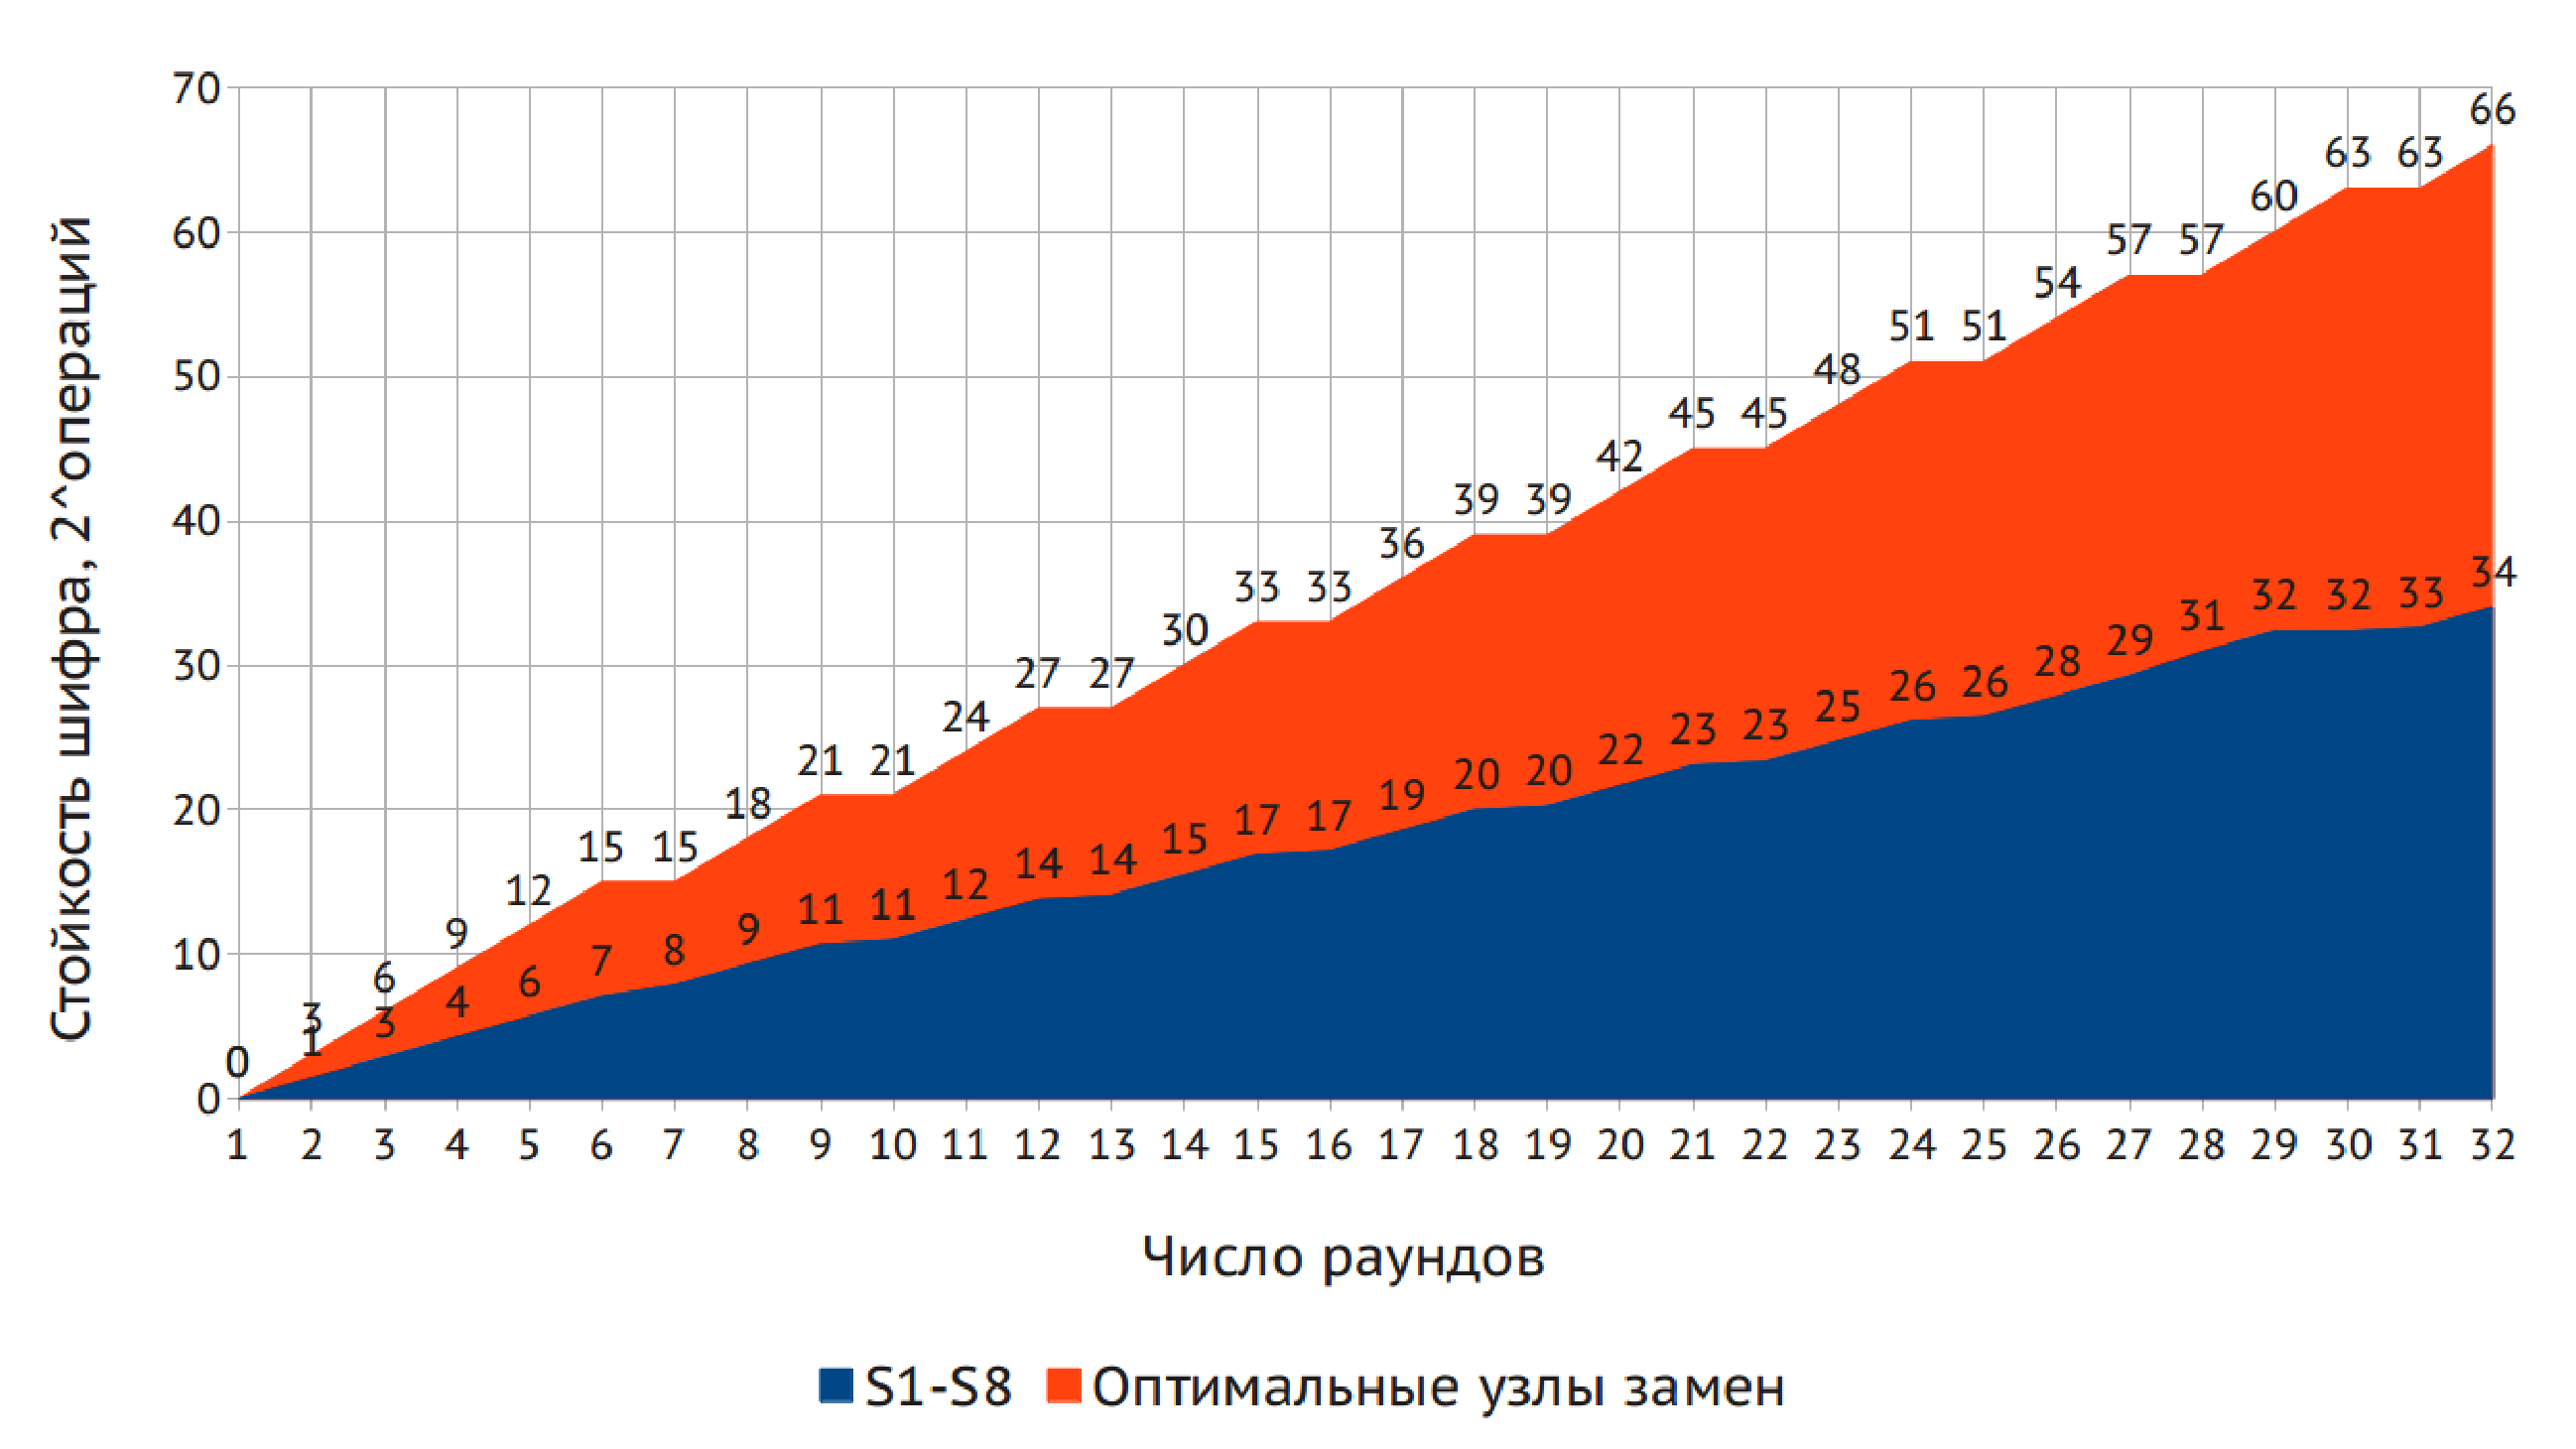
\includegraphics[width=0.8\textwidth]{GOST_diff_efficiency.eps}
    \caption{Зависимость стойкости узлов замен к дифференциальному криптоанализу от числа раундов}
    \label{fig:GOST_diff_efficiency}
\end{figure}

\begin{figure}
    \centering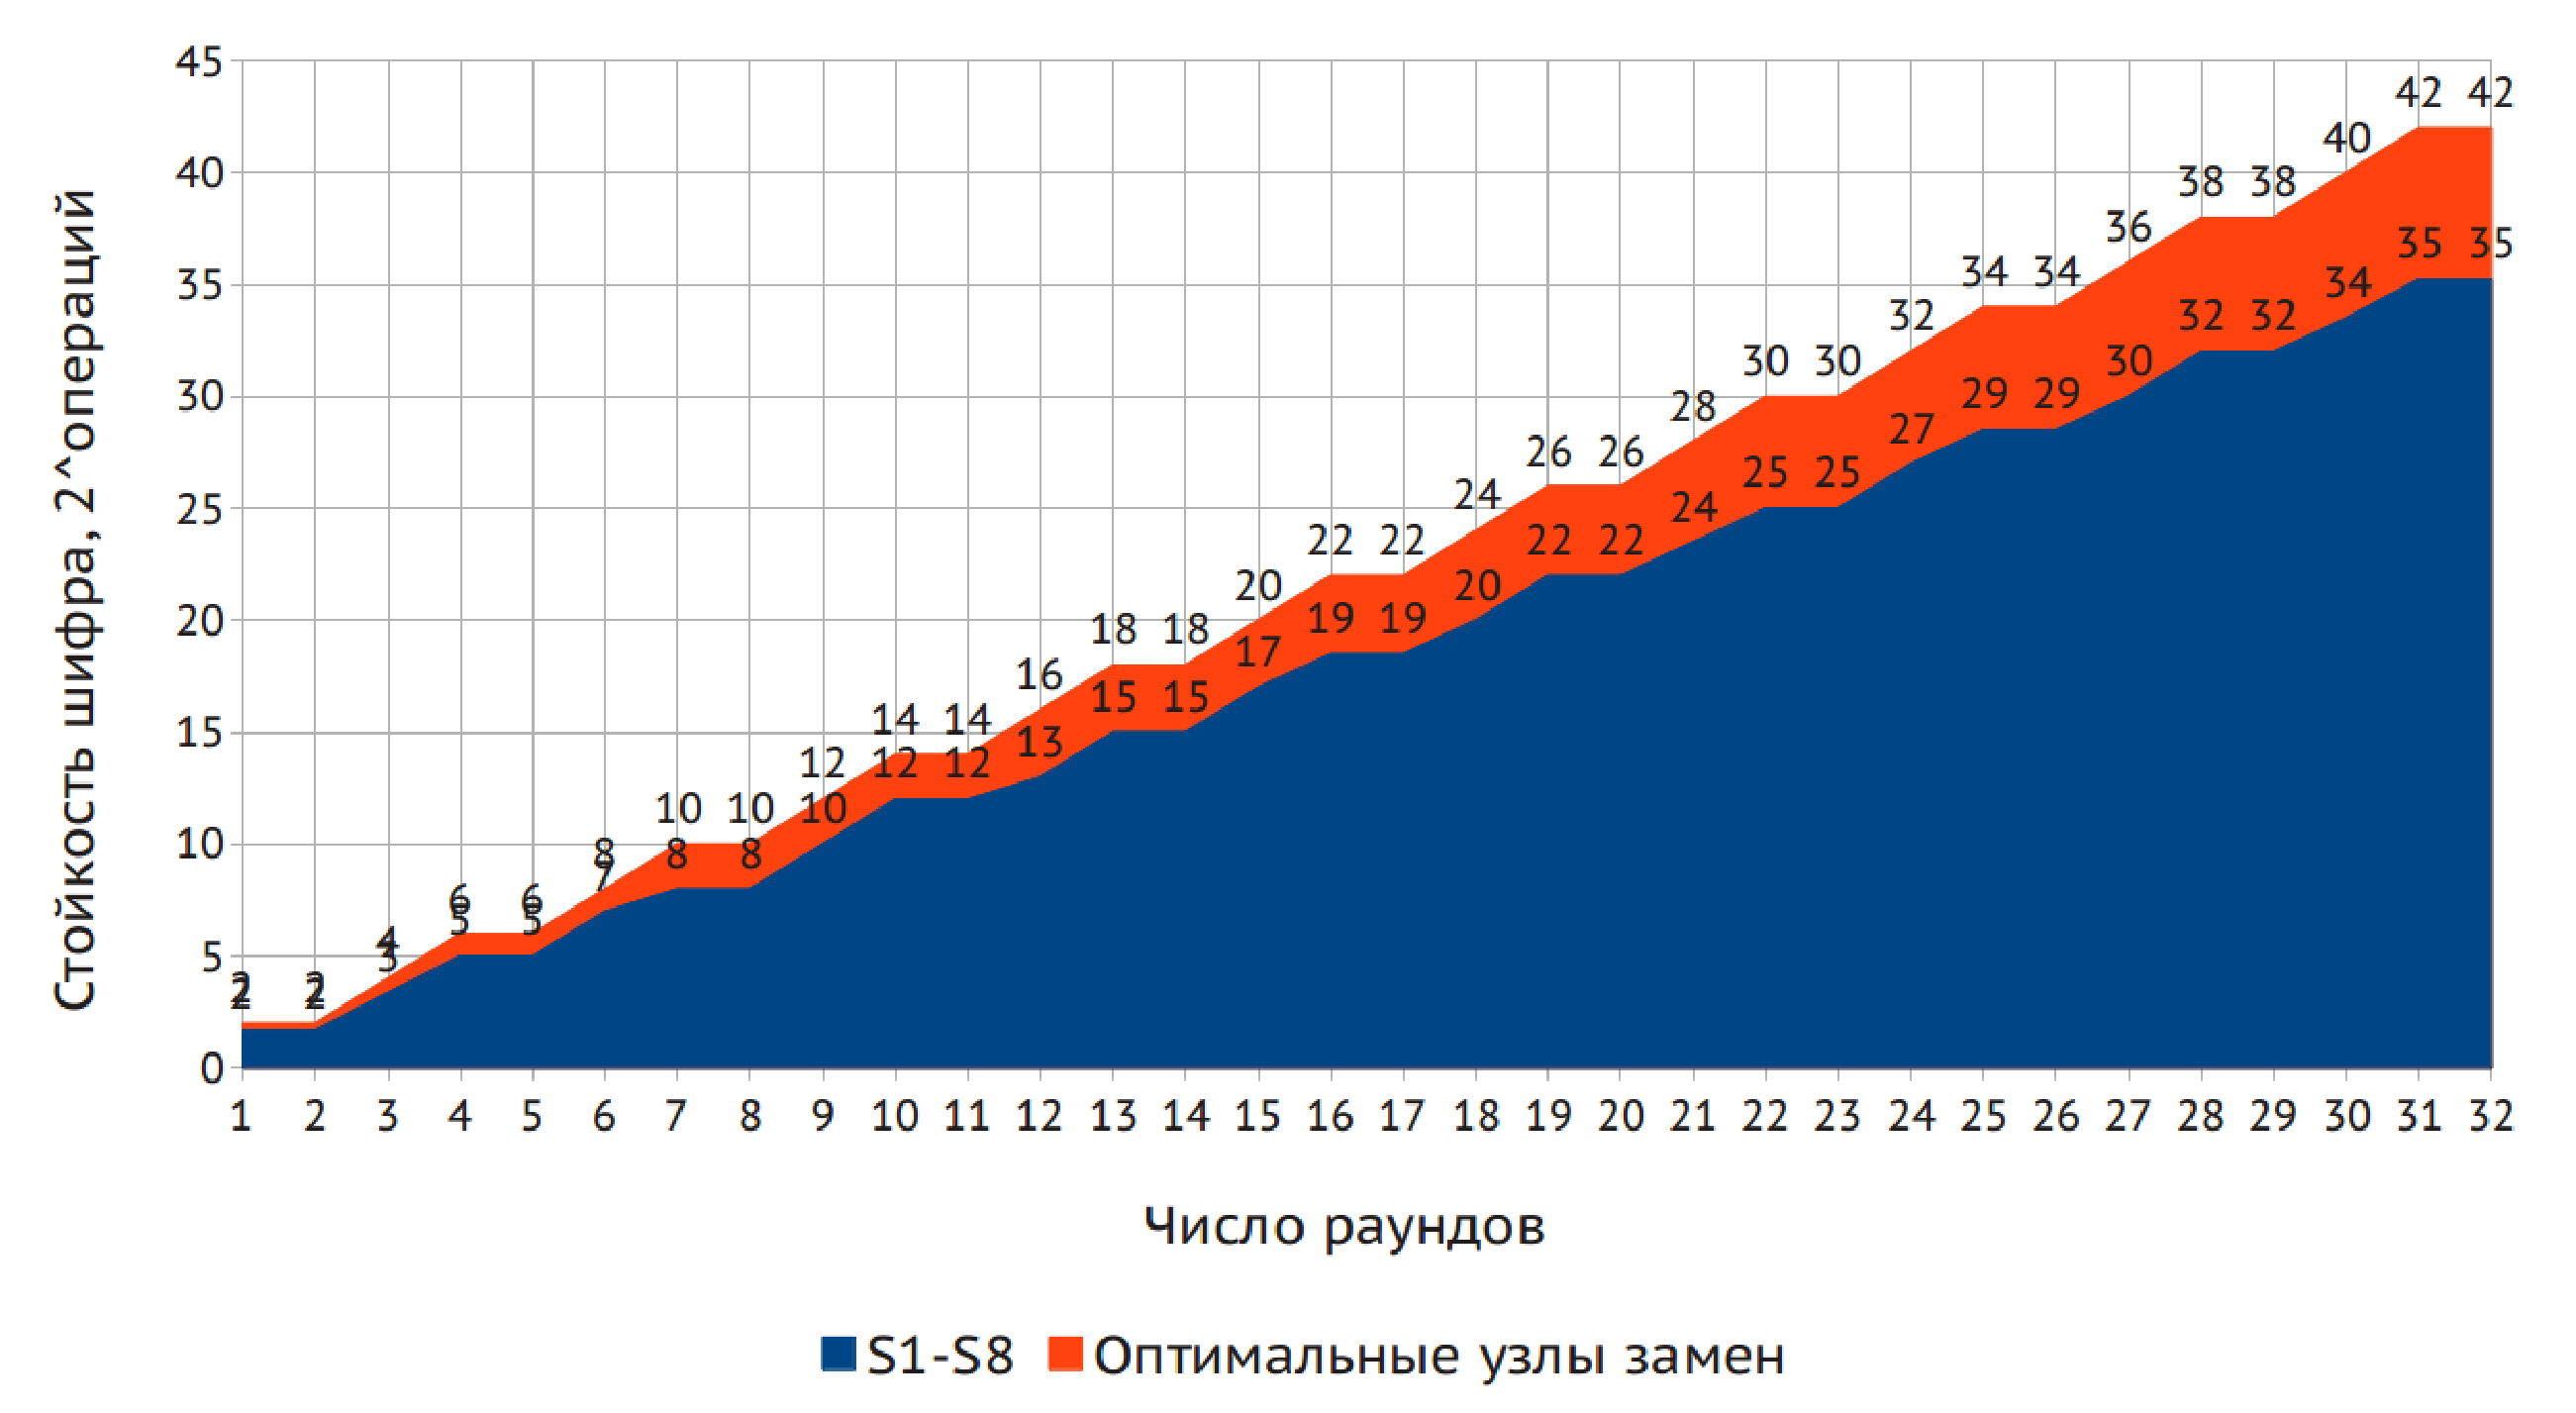
\includegraphics[width=0.8\textwidth]{GOST_linear_efficiency.eps}
    \caption{Зависимость стойкости узлов замен к линейному криптоанализу от числа раундов}
    \label{fig:GOST_linear_efficiency}
\end{figure}

Также стоит отметить скорость получения оптимальных нелинейных узлов замен.
Для сравнения используется наиболее простой альтернативный метод получения узлов
замен "--- метод случайной генерации.

Оценка скорости формирования производилась следующим образом:
\begin{itemize}

    \item устанавливались минимальные удовлетворяющие требования к критериям
    нелинейности, автокорреляции и дифферецниальным и линейным характеристикам;

    \item далее, в течение 48 часов (по 24 часа на каждый метод) на четырёх
    незадействованных серверах были запущены вышеописанные методы формирования
    узлов замен;

    \item по полученным результатам оценивалось количество нелинейных узлов
    замен, прощедших отбор по минимальным требованиям, нормированных на 1
    процесс в сутки "--- K1;

    \item соотношение числа прошедших отбор нелинейных узлов замен к числу
    непрошедших "--- K2.

\end{itemize}

Минимальными удовлетворяющими требованиями были выбраны оптимальные показатели:
\begin{itemize}
    \item нелинейность "--- 4;
    \item автокорреляция "--- 8;
    \item верхняя граница вероятности дифференциального криптоанализа "--- $2^{-66}$;
    \item верхняя граница вероятности линейного криптоанализа "--- $2^{-42}$.
\end{itemize}

Как видно из таблицы~\ref{table:speedtest_GOST_annealing}, метод имитации отжига на 200\%
эффективнее случайной генерации по абсолютному количеству формируемых
оптимальных нелинейных узлов замен, а также на 3 порядка эффективнее с точки
зрения операций проверки выдвинутых для тестирования минимальных требований. Так
метод случайно генерации требует в среднем 10000 проверок финальных условий для
получения одного S-блока, удовлетворяющего требованиям, в то время как метод
имитации отжига формирует оптимальный нелинейный узел замен на каждый пятый
выход.

\begin{table}
    \caption{Оценки скорости формирования нелинейных узлов замен ГОСТ 28147-89}
    \label{table:speedtest_GOST_annealing}
    \begin{tabular}{| m{7.7cm} | m{4cm} | m{4cm} |}
        \hline
        Метод                       & K1, \newline S-блоков/сутки    & K2        \\ \hline
        Метод имитации отжига       & 172                   & 0.2       \\ \hline
        Метод случайной генерации   & 53                    & 0.0001    \\ \hline
    \end{tabular}
\end{table}

\begin{table}[ht]
    \caption{Сравнение вероятности криптоанализа оптимальных нелинейных узлов замен с используемыми в ЦБ РФ}
    \label{table:efficiency_GOST} \def\arraystretch{1.15}
    % XXX: >{\columncolor{white}} for each column is the real hack! There are different border widths for colored cells without it :(
    \setlength{\arrayrulewidth}{1pt}
    \setlength\doublerulesep{1pt}\doublerulesepcolor{white}
    \begin{tabular}{|>{\columncolor{white}} m{1.4cm} |>{\columncolor{white}} m{2.75cm} |>{\columncolor{white}} m{4cm} ||>{\columncolor{white}} m{2.75cm} |>{\columncolor{white}} m{4cm} |}
        \hline
        № раунда    & $M_D(S1-S8)$  & $M_D(\mbox{оптимальные})$         & $M_L(S1-S8)$  & $M_L(\mbox{оптимальные})$         \\ \hline
        1           & $2^0$         & $2^0$                             & $2^{-1.68}$   & $2^{-2}$                          \\ \hline
        2           & $2^{-1.42}$   & $2^{-3}$                          & $2^{-1.68}$   & $2^{-2}$                          \\ \hline
        3           & $2^{-2.83}$   & $2^{-6}$                          & $2^{-3.36}$   & $2^{-4}$                          \\ \hline
        4           & $2^{-4.25}$   & $2^{-9}$                          & $2^{-5.03}$   & $2^{-6}$                          \\ \hline
        5           & $2^{-5.66}$   & $2^{-12}$                         & $2^{-5.03}$   & $2^{-6}$                          \\ \hline
        6           & $2^{-7.08}$   & $2^{-15}$                         & $2^{-6.71}$   & $2^{-8}$                          \\ \hline
        7           & $2^{-7.86}$   & $2^{-15}$                         & $2^{-8.39}$   & $2^{-10}$                         \\ \hline
        8           & $2^{-9.28}$   & $2^{-18}$                         & $2^{-8.39}$   & $2^{-10}$                         \\ \hline
        9           & $2^{-10.69}$  & $2^{-21}$                         & $2^{-10.07}$  & $2^{-12}$                         \\ \hline
        10          & $2^{-10.96}$  & $2^{-21}$                         & $2^{-11.75}$  & $2^{-14}$                         \\ \hline
        11          & $2^{-12.37}$  & $2^{-24}$                         & $2^{-11.75}$  & $2^{-14}$                         \\ \hline
        12          & $2^{-13.79}$  & $2^{-27}$                         & $2^{-13.42}$  & $2^{-16}$                         \\ \hline
        13          & $2^{-14.05}$  & $2^{-27}$                         & $2^{-15.10}$  & $2^{-18}$                         \\ \hline
        14          & $2^{-15.47}$  & $2^{-30}$                         & $2^{-15.10}$  & $2^{-18}$                         \\ \hline
        15          & $2^{-16.88}$  & $2^{-33}$                         & $2^{-16.78}$  & $2^{-20}$                         \\ \hline
        16          & $2^{-17.14}$  & $2^{-33}$                         & $2^{-18.46}$  & $2^{-22}$                         \\ \hline
        17          & $2^{-18.56}$  & \cellcolor[gray]{0.9} $2^{-36}$   & $2^{-18.46}$  & $2^{-22}$                         \\ \hline
        18          & $2^{-19.97}$  & $2^{-39}$                         & $2^{-20.14}$  & $2^{-24}$                         \\ \hline
        19          & $2^{-20.24}$  & $2^{-39}$                         & $2^{-21.81}$  & $2^{-26}$                         \\ \hline
        20          & $2^{-21.65}$  & $2^{-42}$                         & $2^{-21.81}$  & $2^{-26}$                         \\ \hline
        21          & $2^{-23.07}$  & $2^{-45}$                         & $2^{-23.49}$  & $2^{-28}$                         \\ \hline
        22          & $2^{-23.33}$  & $2^{-45}$                         & $2^{-25.17}$  & $2^{-30}$                         \\ \hline
        23          & $2^{-24.74}$  & $2^{-48}$                         & $2^{-25.17}$  & $2^{-30}$                         \\ \hline
        24          & $2^{-26.16}$  & $2^{-51}$                         & $2^{-26.85}$  & $2^{-32}$                         \\ \hline
        25          & $2^{-26.42}$  & $2^{-51}$                         & $2^{-28.53}$  & $2^{-34}$                         \\ \hline
        26          & $2^{-27.84}$  & $2^{-54}$                         & $2^{-28.53}$  & $2^{-34}$                         \\ \hline
        27          & $2^{-29.25}$  & $2^{-57}$                         & $2^{-30.21}$  & \cellcolor[gray]{0.9} $2^{-36}$   \\ \hline
        28          & $2^{-30.93}$  & $2^{-57}$                         & $2^{-31.88}$  & $2^{-38}$                         \\ \hline
        29          & $2^{-32.35}$  & $2^{-60}$                         & $2^{-31.88}$  & $2^{-38}$                         \\ \hline
        30          & $2^{-32.35}$  & $2^{-63}$                         & $2^{-33.56}$  & $2^{-40}$                         \\ \hline
        31          & $2^{-32.61}$  & $2^{-63}$                         & $2^{-35.24}$  & $2^{-42}$                         \\ \hline
        32          & \cellcolor[gray]{0.9} $2^{-34.02}$  & $2^{-66}$   & \cellcolor[gray]{0.9}$2^{-35.24}$  & $2^{-42}$    \\ \hline
    \end{tabular}
\end{table}
